% 第5章
\section{実装(\textcolor{orange}{14\%})}
  \label{sec:実装}
    \par
  
  \subsection{スマートロックの実装(0\%)}
    \label{sec:スマートロックの実装}
      \par
  
      \subsubsection{プロトタイプ作成(0\%)}
        \label{sec:プロトタイプ作成}
          \par
          
      \subsubsection{動作確認(0\%)}
        \label{sec:動作確認}
          \par
          
  \subsection{数理最適化モデルの実装(0\%)}
    \label{sec:数理最適化モデルの実装}
      \par
      
      \subsubsection{ソルバーの選定(\textcolor{green}{100\%}))}
        \label{sec:ソルバーの選定}
          \par ソルバーの性能は,結果の質や計算時間に大きく影響するため,自転車割り当て問題を効率的かつ正確に解くためには適切なソルバーの選定が必要不可欠である.特に,CtoCシェアサイクルシステムにおいては,リアルタイム性やスケーラビリティが求められるため,最適なソルバー選定がシステム全体のパフォーマンスを左右する.
          
          \par 本研究で扱っている自転車割り当て問題の特徴としては,整数線形計画問題として定式化される点が最大の特徴として挙げられる.他にも,変数にはバイナリ値のみが含まれ,制約条件は線形である点も特徴として挙げられる.問題の規模感としては,シェアリングの対象となる自転車の数やユーザの需要などに応じて決定変数である二値変数行列の成分の数が大規模になる可能性も考えられる.そのような状況下においても最適な自転車をユーザに割り当てる必要があるため,解の精度は高く保たれる必要がある.さらに,リアルタイム性が求めらる点も考慮すると,迅速な計算処理を継続して行う必要もある.
          
          \par そこで,ソルバーを選定するにあたって,上記の要件を満たすための観点をいくつかまとめる.まず性能面において,大規模問題でも迅速に解を求められ,効率的なメモリ管理が可能であることや,整数線形計画問題に対応していることが求められる.また,利便性の面において,無料で利用可能であることや,アルゴリズムの実装の際に用いるOR-Toolsとの互換性も求められる.なお,OR-ToolsとはGoogle社から提供されている組み合わせ最適化向けのオープンソースソフトウェアであり,非常に広範な可能性のあるソリューションの中から問題に対する最適化ソリューションを見つけ出すことをサポートする\scalebox{0.7}{\cite{OR-Tools}}.
          
          \par 具体的なソルバーの例として,CPLEXやGurobiなどが挙げられる.CPLEXはIBM社から提供されている,混合整数計画法のための分散型並列アルゴリズムと,線形計画,混合整数計画などのための柔軟で高性能な数理計画法ソルバーである\scalebox{0.7}{\cite{CPLEX}}.GurobiはGurobi社から提供されているソルバーであり,並列処理を最大限活用するよう構築され,高度なMIPヒューリスティックアルゴリズムにより実現可能解を素早く求解可能である特徴を持つ\scalebox{0.7}{\cite{Gurobi}}.しかし、これらのソルバーはオープンソースではないが故に,ライセンス費用の面における制限が懸念される.
          
          \par オープンソースソルバーの例としては,GLPKやCBCなどが挙げられる.
          
          \par GLPKはモスクワ航空大学のAndrew Makhorin氏によって開発されたソルバーである.C言語で記述されており,コマンドラインまたはAPIを介して操作可能であり,CとJavaのAPIを提供している.CPLEXのような商用ソルバーと比較するとGLPKの速度は劣るものの,線形計画問題に対して有効なソルバーである\scalebox{0.7}{\cite{gearhart2013comparison}}.
          
          \par CBCはJohn Forrest氏らによって開発された,COIN-OR線形計画法を用いた混合整数計画問題を解くためのソルバーである.C++で書かれており,呼び出し可能なライブラリとしても,スタンドアロンの実行ファイルとしても利用可能である.様々なモデリングシステムやパッケージなどを通して,様々な方法で利用することができる\scalebox{0.7}{\cite{CBC}}.
          
          \par また,オープンソースソルバーの別の例としてSCIPも挙げられる.SCIPは,混合整数線形計画問題や混合整数比線形計画問題,さらには制約整数計画問題のソルバーとして設計された,制約整数計画ソルバーである\scalebox{0.7}{\cite{bolusani2024scip}}.SCIPソルバーは汎用性の高いフレームワークであり,問題のサイズを縮小する前処理や下界値を強化するカット生成,より良い上限値を与えるためのヒューリスティック解法などの機能をプラグインとして追加することができる.これによってSCIPソルバーの利用者は問題に合わせてカスタマイズし,性能を向上させることができる\scalebox{0.7}{\cite{shinano2013CIPSolver}}.一方で,SCIPを利用することの欠点としては,高機能であるが故に複雑性が高く,ある程度の学習コストを要する点や,多数のパラメータを持ち,その設定によって性能が大きく変化するため,最適なパラメータを見つけるためのチューニングが難しい場合がある.
          
          \par 上記で述べた要件やソルバーの一長一短を鑑み,本研究ではSCIPを自転車割り当てにおける整数線形計画問題のソルバーとして選定する.選定理由の最も大きなポイントとしては,オープンソースのソルバーであり,利用するにあたってライセンス関連のコストを懸念する必要が無い点である.オープンソースソルバーとしてSCIP以外に挙げたGLPKやCBCと比較して計算速度が優位である点もSCIPを選定したポイントの1つである.さらに,アルゴリズムの実装の際に用いるOR-Toolsとの互換性が高い点も選定ポイントとして挙げられる.SCIPを利用する際のデメリットとして挙げた複雑性について,OR-Toolsを併用して利用した場合,比較的シンプルにアルゴリズムを実装することが可能となるため,SCIPの長所を最大限生かした実装を行えることが期待される.
          
      \subsubsection{アルゴリズムの実装(\textcolor{green}{100\%})}
        \label{sec:アルゴリズムの実装}
          \par 本研究で提案する数理最適化ベースの自転車割り当てアルゴリズムは,単にユーザの最短距離に配置されている自転車を割り当てるわけではない.複数のリクエストをストックした上で,\ref{sec:数理最適化モデルの定式化}項で定義した目的関数や制約条件のもと,ユーザの移動後の自転車の配置が全体最適となるように割り当てることによって,CtoCシェアサイクルサービスを実現させることを目的としている.
          \par そこで,実際に\ref{sec:ソルバーの選定}項にて選定したSCIPソルバーを用いて数理最適化ベースの自転車割り当てモデルをモジュールとして実装する.実装する際にはプログラミング言語Pythonを利用する.Pythonとは,1991年にGuido van Rossum氏によって開発されたプログラミング言語であり,コードの可読性を重視した設計哲学や動的型付け言語でありコンパイルが不要である点,包括的な標準ライブラリがサポートされている点などが特徴として挙げられる\scalebox{0.7}{\cite{aboutPython}}.その他,主要なライブラリ及びパッケージとしてSciPyやNumpy,Pandasなどを用い,開発環境としてGoogle Colaboratoryを利用する.
          \par ユーザリクエストをストックするために定義されるある時間幅に対して処理を実行するアルゴリズム全体のフローチャートは図\ref{fig:自転車割り当てアルゴリズムのフローチャート}で示す通りである.ただし,割り当てモデルクラスをインスタンス化する際のパラメータとして,データフレーム型の地理情報データとシェアリングされる自転車データ$B$を指定する.そうすることによって,指定された地域の特性や利用可能な自転車の数,及びステータスに対して柔軟に対応可能となる.なお,ここで用いる記号で説明を省略している場合は,表\ref{tab:記号の概説}の通りとする.
          \par 距離行列の生成では,入力されるリクエストデータや自転車のステータスから自転車の現在地や自転車の所有者までの位置,ユーザの現在地などの位置情報を取得し, 測地線距離を用いてそれぞれの対象間の距離を計算し,行列として値を格納する.測地線距離とはリーマン多様体上の2点間の最短経路の長さとして定義\scalebox{0.7}{\cite{shuvo2024geodesic}}され,空間の曲率を考慮した距離を算出する.さらに,距離のスケールを統一するため,生成した距離行列に対してデータの平均が0,標準偏差が1になるよう正規化を実施する.これにより,モデルクラスをインスタンス化する際の地理情報データに依存せず,一貫性を持ったパラメータの調整を行うことができる.
          \par 利用可能な自転車$B_{\text{able}}$は二値行列であり,リクエストされた時刻とシェアリング対象自転車の集合$B$の貸し出し終了日時カラムの値を元に生成される.貸し出し終了日時がNullまたはリクエストされた時刻より過去である自転車は現在利用可能であると判定され1を格納し,それ以外の場合は0を格納する.
          \par データの取得・整形後に数理最適化を実行し,自転車とユーザの割り当て解が存在するか否かを確認する.解が存在しない場合は処理を終了する.解が存在する場合は,その割り当て解を返し,さらに,シェアリング対象自転車の集合$B$の割り当てられたそれぞれの自転車に対して貸し出し終了日時カラムの値をユーザリクエストの情報を元に更新する.以降,シェアリング対象自転車の集合$B$を取得する際に,更新された自転車のステータスを元に$B_{\text{able}}$の取得処理が繰り返される.
          \par より大規模なリクエストデータ及び自転車データに対して自転車割り当てアルゴリズムを適用する場合,計算処理に多くのコストを要し,レスポンスまでの待機時間が大幅に上昇する場合がある.レスポンスまでの時間が増大するとユーザ体験は著しく低下し兼ねない.そのため,必要に応じてPythonによるGPU高速計算のためのオープンソースの配列ライブラリCuPyを利用する.CuPyのインターフェースはNumPyと高い互換性を持ち,NumPy配列を定義・利用している箇所をCuPyに置き換えるだけでGPUで並列処理を適切に実行することができ,レスポンスまでの時間を縮小することができる\scalebox{0.7}{\cite{CuPy}}.
          \par エラーハンドリングとして,モデルに入力される値に対しての例外処理を実装する.例えば,インスタンス化する際に入力されるデータフレーム型の地理情報データの経度・緯度カラムに有効な値が格納されているかや,リクエストデータが有効なデータフレームであるかなどの観点が挙げられる.条件分岐による例外出力や随時デバッグ出力にて確認できるよう構築する.

          \begin{figure}[htbp]
            \centering
            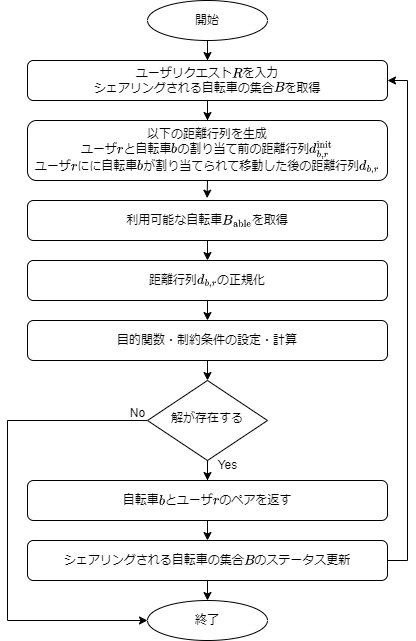
\includegraphics[scale=0.55]
            {figures/algorithmImplementation.png}
            \caption{自転車割り当てアルゴリズムのフローチャート}
            \label{fig:自転車割り当てアルゴリズムのフローチャート}
          \end{figure}

      \subsubsection{テストケースと結果(0\%)}
        \label{sec:テストケースと結果}
          \par  
  
  \subsection{機械学習モデルの実装(0\%)}
    \label{sec:機械学習モデルの実装}
      \par 
      
      \subsubsection{データセットの準備(0\%)}
        \label{sec:データセットの準備}
          \par
          
      \subsubsection{特徴量の選択と前処理(0\%)}
        \label{sec:特徴量の選択と前処理}
          \par
          
      \subsubsection{モデルの学習と評価(0\%)}
        \label{sec:モデルの学習と評価}
          \par
          
  \subsection{API開発(0\%)}
    \label{sec:API開発}
      \par
      
      \subsubsection{APIエンドポイントの実装(0\%)}
        \label{sec:APIエンドポイントの実装}
          \par
          
      \subsubsection{ドキュメンテーションとテスト(0\%)}
        \label{sec:ドキュメンテーションとテスト}
          \par
